\documentclass[final]{beamer}

% ====================
% Packages
% ====================

\usepackage[T1]{fontenc}
\usepackage{lmodern}
\usepackage[size=a0,orientation=portrait,scale=1.2]{beamerposter}
\usetheme{AISystemsLab}
\usecolortheme{AISystemsLab}
\usepackage{graphicx}
\usepackage{booktabs}
\usepackage{tikz}
\usetikzlibrary{positioning, calc}
\usepackage{pgfplots}
\pgfplotsset{compat=1.17}
\usepackage{adjustbox}

% ====================
% Lengths
% ====================

% If you have N columns, choose \sepwidth and \colwidth such that
% (N+1)*\sepwidth + N*\colwidth = \paperwidth
\newlength{\sepwidth}
\newlength{\colwidth}
\setlength{\sepwidth}{0.025\paperwidth}
\setlength{\colwidth}{0.3\paperwidth}

\newcommand{\separatorcolumn}{\begin{column}{\sepwidth}\hspace{0.0125\paperwidth}\raisebox{-\height}[0pt][0pt]{\begin{tikzpicture} \draw[dash pattern=on 2pt off 8 pt, ultra thick](0,86) -- (0,0); \end{tikzpicture}}\end{column}}

\newcommand{\separatorcolumnwithoutline}{\begin{column}{\sepwidth}\end{column}}

\newcommand{\separatorblocks}{\vspace{-25 pt}\begin{block}{}\begin{tikzpicture}\draw[dash pattern=on 2pt off 8pt, ultra thick](0,0) -- (22,0); \end{tikzpicture}\end{block}}

% ====================
% Title
% ====================

\title{Ultra-Wideband (UWB) Positioning System\\Based on ESP32 and DWM3000 Modules}

\author{T. Herter \and S. Krebs}
\institute[AI Systems Lab]{AI Systems Lab}

% ====================
% Footer (optional)
% ====================

\footercontent{
  sourcecode:
  
\includegraphics[scale=0.3]{pics/qr_link_repo.png} \hfill
  \hfill
  \parbox{30em}{ Hochschule Konstanz Technik, Wirtschaft und Gestaltung \\ Departement of Electrical Engineering and Information Technology }
}
% (can be left out to remove footer)

% ====================
% Body
% ====================

\begin{document}
\addtobeamertemplate{headline}{}
{
    \begin{tikzpicture}[remember picture,overlay]
      \node [anchor=north west, inner sep=3cm] at ([xshift=-4cm,yshift=1.0cm]current page.north west)
      {
\includegraphics[height=13.0cm]{pics/HTWG_EI_en_Modul_Zusatz_neg_1C.png}
      }; % also try shield-white.eps
      \node [anchor=north east, inner sep=3cm] at ([xshift=3.0cm,yshift=1.5cm]current page.north east)
     {
\includegraphics[height=7.0cm]{pics/HTWG_EI_Modul_Zeichen_neg_2C.png}
      };
    \end{tikzpicture}
}

\begin{frame}[t]
\begin{columns}[t]
\separatorcolumnwithoutline

\begin{column}{\colwidth}

  \begin{block}{Introduction}
    Indoor positioning and tracking systems gain importance in a variety of industrial fields as well as in research.

    Traditional positioning systems, however, often encounter certain limitations, such as accuracy to the meter or an increased positioning deviation. 

    To achive an improved accuracy and a reduced variance Ultra-Wideband (UWB) positioning systems have been applied to various scenarios.
    Building on this technology, we have developed an UWB positioning system that utilizes hardware and advanced algorithms to generate precise position information in the three-dimensional space.
    However, the estimations that are conducted over the course of its development are limited to the two-dimensional space. 

    The designed UWB system consists of six identical boards that are all based on the ESP32 microcontroller, a versatile and powerful platform that is often used in low-cost IoT scenarios. 
    These custom-made PCB's are equipped with DWM3000 modules from Quorvo, which utilizes UWB functionalities for short-range wireless communication.

    One of these boards is referred to as a ''tag''.
    It is responsible for initiating measurements with the other five "anchor" boards.
    The innovative aspect of the system lies in its ability to perform accurate localization without dependence on external infrastructure for its processing,
    since all the necessary calculations are performed on the device itself that is being localized.
    \end{block}
  \separatorblocks
  
  \begin{block}{Hardware}
    The hardware design of UWB boards draws inspiration from pre-existing DWM3000 evaluation
  boards.
  However, the proprietary board development enables specialized component selection, tailored to their intended use cases.
  User-friendliness was a paramount consideration during the design process,
  resulting in the integration of multiple user buttons and indicating LEDs for versatile purposes like triggering the initialization of the bluetooth server, in order to view or change the stored anchor positions. 
  Additionally, the PCB incorporates a convenient on-board LiPo battery charging and protection circuit via USB-C interface.

  \begin{figure}[hbt!]
    \centering
    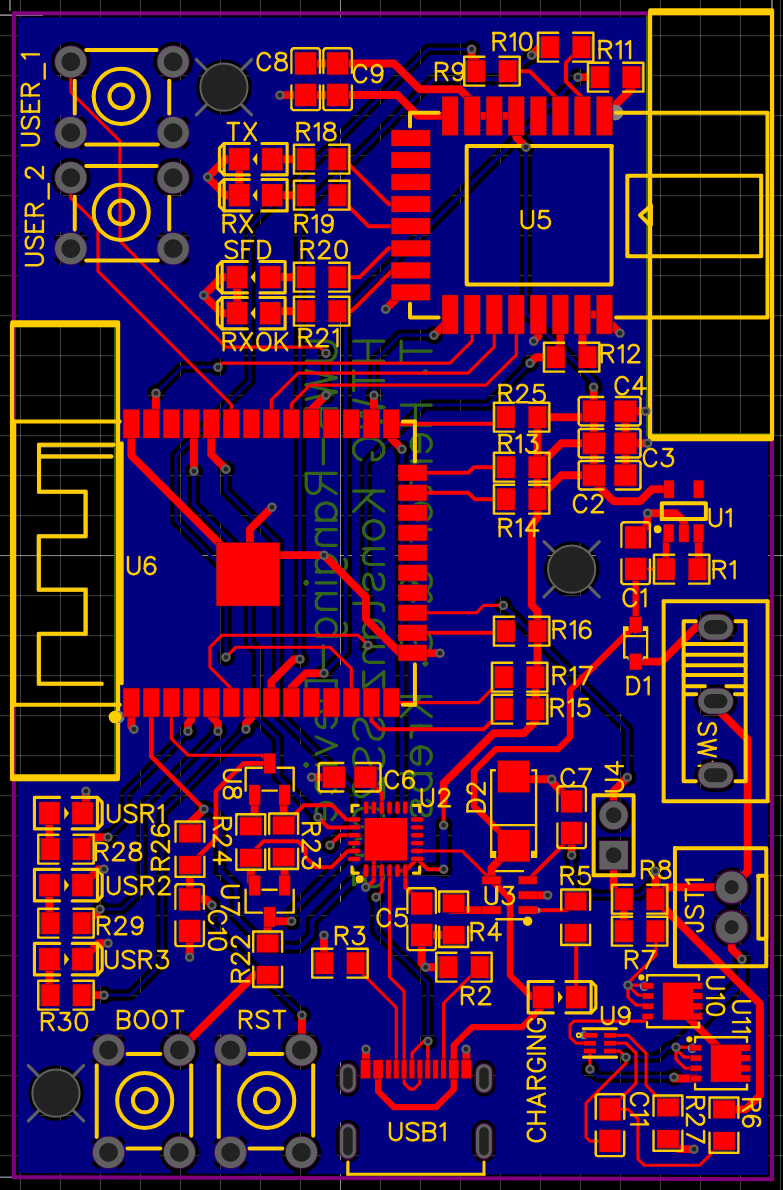
\includegraphics[scale=0.60, angle=90]{pics/pcb_design.png}
    \caption{PCB layout of the UWB board.}
    \label{fig:pcb}
  \end{figure}

  As shown in figure \ref{fig:pcb}, the board is designed in a compact form,
  making it suitable for evaluation and development purposes.
  Notably, our PCB design ensures a consistent layout across all boards, regardless of their specific application.
  Below the antennas of both the DWM3000 and ESP32, the ground filling has been selectively omitted, to ensure antenna radiation characteristics according to the corresponding data sheets, enabling more precise measurements.
  \end{block}
\end{column}

\separatorcolumn

\begin{column}{\colwidth}

  \begin{block}{Two-way-Ranging (TWR)}
    TWR is a foundational technique for obtaining precise distance measurements
    within the UWB positioning system.
    It relies on the time it takes for signals to propagate from a tag board
    to an anchor board and back again.
    This time measurement, in compliance with the IEEE 802.15.4a/4z standards,
    offers the basis for distance estimation by multiplying the time traveled with the speed of light.

    \begin{figure}[H]
      \begin{tikzpicture}[
        node distance=1.5cm,
        block/.style={
          align=center, draw,line width=0.5mm, minimum width=6.85cm, minimum height=.5cm
        },
        ghost/.style={
          align=center,minimum width=0cm, minimum height=0cm
        },
        label/.style={
          minimum width=6cm, minimum height=0cm, text width=6cm
        },
        >=latex,
      ]
        % textfields
        \node [block] (tag_timestamp) {Tag\\Timestamp};
        \node [block, right=2cm of tag_timestamp] (anchor_timestamp) {Anchor\\Timestamp};
    
        % Endpoints
        \node [ghost, below=8cm of tag_timestamp] (tag_endpoint) {};
        \node [ghost, below=8cm of anchor_timestamp] (anchor_endpoint) {};
    
        % Timelines
        \draw [line width=0.5mm, -] (tag_timestamp) -- (tag_endpoint);
        \draw [line width=0.5mm, -] (anchor_timestamp) -- (anchor_endpoint);
    
        % Labels Tag-line
        \node [label, align=right, anchor=east, below=2cm of tag_timestamp.west] (t_send_poll) {$t_{send-poll}$\\$(t_{sp})$};
        \node [label, align=right, anchor=east, below=7cm of tag_timestamp.west] (t_receive_response) {$t_{receive-response}$\\$(t_{rr})$};
        
        % Labels Anchor-line
        \node [label, align=left, anchor=west, below=3cm of anchor_timestamp.east] (t_receive_poll) {$t_{receive-poll}$\\$(t_{rp})$};
        \node [label, align=left, anchor=west, below=6cm of anchor_timestamp.east] (t_send_response) {$t_{send-response}$\\$(t_{sr})$};
    
        %Dotted lines
        \draw [line width=0.5mm, ->] (t_send_poll.east) -- (t_receive_poll.west);
        \draw [line width=0.5mm, ->] (t_send_response.west) -- (t_receive_response.east);
        \node [ghost, below=2.25cm of anchor_timestamp.west] (poll_label) {Poll (ID)};
        \node [ghost, below=6.5cm of tag_timestamp.east] (response_label) {Response};
    
      \end{tikzpicture}
      \caption{Timingdiagram of Two-Way-Ranging}
    \end{figure}

    The tag's firmware calculates the TOF as well as the distance
    between both devices by comparing the timestamps of sending and reception. 
    Therefore it is necessary for the UWB messages to not only be tracked by
    the time they are received at the tag,
    but also to contain information about when each anchor received it and when
    it starts to transmit the response.

    \begin{equation*}
      \begin{aligned}
        t_{tof} &= \frac{(t_{rp} - t_{sp})+(t_{rr} - t_{sr})}{2}\\
        dist &= t_{tof} * v_{light}\\
        v_{light} &\approxeq 299.792.458,0 \frac{m}{s}
      \end{aligned}
    \end{equation*}

    Using this technique the standarddeviation of die distance estimation
    is approximatly between 4cm to 10cm, depending on the conditions of measurement.
    The estimation error increases significantly if there is a non-line-of-sight condition.

  \end{block}

  \separatorblocks

  \begin{block}{Firmware}
    The Firmware for both the Tags and Anchors shares a common codebase
    with only a minor distinction during device startup.
    Upon booting, the current role of the device is read from the EEPROM,
    and based on this role, the appropriate tasks are executed.

    The development of firmware built on FreeRTOS offers the capability
    to seemingly execute multiple tasks in parallel.
    Leveraging the dual cores of the ESP32 microcontroller allows us to
    genuinely achieve parallelism.

    This design approach ensures efficient resource utilization and
    effective task management, ultimately contributing to the system's
    overall performance.
  \end{block}

  \begin{alertblock}{Firmware Tasks:}
    \begin{itemize}
      \item \textbf{TOF-Task}: used for executing UWB measurements, eather as Initator or as Responder.
      \vspace*{1cm}
      \item \textbf{EKF-Task}: combines Distance measurements and creates a position estimation.
      \vspace{1cm}
      \item \textbf{BLE-Task}: opens up a Bluetooth server which serves as configuration and feedback interface.
      \vspace{1cm}
    \end{itemize}
  \end{alertblock}
\end{column}

\separatorcolumn

\begin{column}{\colwidth}

  \begin{block}{Extended-Kalman-Filter}
    The Kalman filter primarily consists of three steps.
    First, the state for the next timeiteration is predicted based on the
    current estimated state.
    Next, a measurement is predicted based on the predicted state.
    Finally, the actual measurement is compared to the predicted measurement,
    and the state estimation is corrected based on the estimation error.
    This process leads to the convergence of the estimation towards the ground truth.

    The following blockdiagram shows how the different steps interact to generate a
    state estimation based on the current measurement.
    
    \begin{figure}
      \hspace*{-1.25cm}
      \begin{tikzpicture}[
          node distance=1.5cm,
          block/.style={
              rectangle, draw, align=center,
              minimum width=3cm, minimum height=1.5cm,
              font =\small
          },
          >=latex,
      ]
          % System block
          \node [block] (system) {system};
          \node [left=10cm of system] (uk) {$u_k$};
          \node [right=9cm of system] (zk1) {$z_{k+1}$};
          \node [left=.5cm of system] (x_k) at (system.south west) {$x_{k}$};
          \node [right=.5cm of system] (x_k1) at (system.south east) {$x_{k+1}$};
      
          % Kalman filter blocks
          \node [block, below=3cm of system] (messmodel) {measurement-\\modell};
          \node [block, left=2.5cm of messmodel] (systemmodel) {system-\\modell};
          \node [block, right=3.5cm of messmodel] (correction) {correction};
          \node [right=1cm of correction] (x_dach_k1) {$\hat{x}_{k+1}$};
          \node [left=1.5cm of systemmodel] (x_dach_k) at (systemmodel.south west) {$\hat{x}_{k}$};
  
          % Arrows
          \draw [line width=0.5mm, ->] (uk) -- (system);
          \draw [line width=0.5mm, ->] (system.east) -- ++(.5,0) |- (zk1);
      
          \coordinate[right=-9cm of system.west] (systemcoord_left);
          \draw [line width=0.5mm, ->] (systemcoord_left) |- (systemmodel.west);
          \draw [line width=0.5mm, ->] (systemmodel.east) -- node[above] {$\hat{x}_{k+1|k}$} (messmodel.west);
          \draw [line width=0.5mm, ->] (messmodel.east) -- node[above] {$\hat{z}_{k+1|k}$} (correction.west);
      
          \coordinate[right=1cm of correction.east] (correctioncoord);
          \draw [line width=0.5mm, ->] (correction.east) -- ++(1,0);
          \coordinate[right=2.5cm of system.east] (systemcoord_right);
          \draw [line width=0.5mm, ->] (systemcoord_right)
              |- ($(systemcoord_right)+(3,0)$)
              |- ($(correction.west)+(-.5,3)$)
              |- ($(correction.west)+(-.5,2)$)
              |- ($(correction.west)+(0,.5)$);
  
          \draw [line width=0.5mm, ->] ($(system.east)+(0,-.5)$)
              |- ($(system.east)+(.75,-0.5)$)
              |- ($(system.east)+(.75,-1.5)$)
              |- ($(system.west)+(-.75,-1.5)$)
              |- ($(system.west)+(-.75,-.5)$)
              |- ($(system.west)+(0,-.5)$);
  
          \draw [line width=0.5mm, ->] (messmodel.west)
              |- ($(messmodel.west)+(-1,0)$)
              |- ($(messmodel.west)+(-1,-2)$)
              |- ($(messmodel.east)+(1,-2)$)
              |- ($(correction.west)+(0,-.5)$);
          
          \draw [line width=0.5mm, ->] (correction.east)
              |- ($(correction.east)+(.5,0)$)
              |- ($(correction.east)+(.5,-2.5)$)
              |- ($(systemmodel.west)+(-1.75,-2.5)$)
              |- ($(systemmodel.west)+(0,-.5)$);
        \end{tikzpicture}
        \caption{Block diagram of the Kalman Filters}
      
    \end{figure}
    %In this context, $u_k$ represents control commands that input into the system.
    %$z_k$ describes the observed measurement at time $k$, and $x$ represents the
    %current system state.
    %In the case of our application, $x$ contains the three-dimensional coordinates
    %of the tag, and the vector $z$ encompasses all distance measurements
    %to the landmarks, which are the anchors.
    %Every time a variable is marked with a hat,
    %that means that this is an estimation of the given variable.
  \end{block}

  \separatorblocks

  \begin{block}{Tests}
    The measurements given in the table below were conducted in a
    laboratory environment under good Line-of-Sight conditions.
    As can be seen, the standard deviation of the position estimation is below 10cm.
    However, the absolut deviation of the position estimation is relatively high.
    This deviation is a result of the Kalman-Filter, trying to solve a three-dimensional
    calculation with a minimum anchor amount and their non-ideal mounting positions.

    \begin{table}[hbt!]
      \centering
      \begin{tabular}{l l l c}
        %\toprule
        \textbf{Position[m]} & \textbf{$\mu$[cm]} & \textbf{$\sigma$[cm]}\\
        $(x,y)$ & $mean(length)$ & $std(length)$\\
        %\midrule
        $(2,2)$ & $67.66$ cm & $2.90$ cm\\
        $(2,3)$ & $55.42$ cm & $2.97$ cm\\
        $(2,4)$ & $65.05$ cm & $2.8$ cm\\
        $(2,5)$ & $47.31$ cm & $3.51$ cm\\
        $(2,6)$ & $46.07$ cm & $3.13$ cm\\
        $(2,7)$ & $54.00$ cm & $3.17$ cm\\
        $(2,8)$ & $34.48$ cm & $3.3$ cm\\
    
        $(3,2)$ & $31.74$ cm & $3.42$ cm\\
        $(3,3)$ & $121.37$ cm & $4.47$ cm\\
        $(3,4)$ & $23.06$ cm & $3.07$ cm\\
        $(3,5)$ & $29.34$ cm & $2.91$ cm\\
        $(3,6)$ & $28.31$ cm & $2.93$ cm\\
        $(3,7)$ & $22.68$ cm & $3.2$ cm\\
        $(3,8)$ & $32.98$ cm & $3.73$ cm\\
    
        $(4,2)$ & $19.75$ cm & $2.97$ cm\\
        $(4,3)$ & $21.73$ cm & $3.4$ cm\\
        $(4,4)$ & $29.91$ cm & $2.9$ cm\\
        $(4,5)$ & $9.27$ cm & $3.2$ cm\\
        $(4,6)$ & $28.1$ cm & $2.84$ cm\\
        $(4,7)$ & $35.95$ cm & $8.34$ cm\\
        $(4,8)$ & $14.88$ cm & $3.13$ cm\\
    
        %$(5,2)$ & $80.12$ cm & $3.61$ cm\\
        %$(5,3)$ & $61.88$ cm & $4.19$ cm\\
        %$(5,4)$ & $47.44$ cm & $3.57$ cm\\
        %$(5,5)$ & $21.28$ cm & $6.76$ cm\\
        %$(5,6)$ & $31.89$ cm & $3.65$ cm\\
        %$(5,7)$ & $33.02$ cm & $3.72$ cm\\
        %$(5,8)$ & $26.27$ cm & $3.73$ cm\\
    
        %$(6,2)$ & $89.12$ cm & $2.99$ cm\\
        %$(6,3)$ & $99.28$ cm & $4.28$ cm\\
        %$(6,4)$ & $73.01$ cm & $3.88$ cm\\
        %$(6,5)$ & $55.42$ cm & $6.16$ cm\\
        %$(6,6)$ & $10.63$ cm & $4.56$ cm\\
        %$(6,7)$ & $29.46$ cm & $7.01$ cm\\
        %$(6,8)$ & $13.0$ cm & $2.86$ cm\\
        
        %\bottomrule
      \end{tabular}
      \caption{Static measurement deviation out of 500 measurements at each grid intersection point.}
      \label{table:measurements}
    \end{table}

    Applying a fixed constraint for the z-axis would reduce the three-dimensional estimation
    to a two-dimensional one.
    This would allow the Kalman-Filter to deliver more precise position estimations.
    Overall this project created an universal platform for further research in the field of UWB positioning and communication.

  \end{block}
\end{column}

\separatorcolumnwithoutline
\end{columns}
\end{frame}

\end{document}